\chapter[Generalidades]{Generalidades sobre la marcha}

El siguiente capítulo pretende introducir al lector los conceptos fundamentales relacionados a la marcha y su estudio. Además de los avances tecnológicos en el área y el estado de estos.

\section{¿Qué es la marcha?}

Por \emph{marcha} se entiende el acto de desplazarse utilizando las extremidades corporales. Para \cite{perry} al caminar se utiliza una secuencia de movimientos de las extremidades, con el fin de mover el cuerpo hacia adelante y mantener la estabilidad. Cada uno de estos ciclos (de la secuencia) involucra la interacción de las dos extremidades inferiores, compuestas de varios segmentos, y la masa total del cuerpo. El estudio de la marcha consiste en la identificación de patrones de movimiento generados en la marcha y la segmentación del ciclo.

Es posible utilizar la física clásica para estudiar la marcha. Se puede describir la cinemática de la marcha al determinar las velocidades y aceleraciones de los segmentos rígidos del cuerpo; también se puede describir la dinámica de la marcha al determinar las fuerzas que actúan sobre los segmentos rígidos. Así, la marcha se estudia de dos maneras principales: el vector de fuerza recíproca generado por el suelo al soportar el peso del cuerpo y las velocidades y aceleraciones de las principales uniones involucradas en la marcha. \citep{perry}

Ambas descripciones, cinemática y dinámica, se pueden utilizar para segmentar el ciclo de la marcha. \citep{perry} lo divide según se muestra en la tabla \ref{tab:ciclo_marcha}, además la figura \ref{fig:ciclo_marcha} muestra imágenes tomadas del mismo autor. 

\begin{table}
    \centering
    \caption{Ciclo de la marcha según \citep{perry}}
    \label{tab:ciclo_marcha}
    \begin{tabular}{l l l}
        \toprule
        Función & Fase & Descripción \\
        \midrule
        Aceptación de la carga & Contacto Inicial & Justo cuando el pie toca el suelo \\
                               & Respuesta a la carga & El otro comienza el balanceo \\
        Soporte & Soporte medio & El centro de masa se alinea con el pié \\
                & Soporte final & El centro de masa sobrepasa el piel \\
        Avance del miembro & pre-balanceo & Se transfiere la carga al otro pie \\
                           & balanceo inicial & Se levanta el pie y avanza \\
                           & balanceo medio   & El pie sobrepasa al otro \\
                           & balanceo final   & Posición apta para contacto inicial \\
        \bottomrule
    \end{tabular}
\end{table}

\begin{figure}
    \centering
    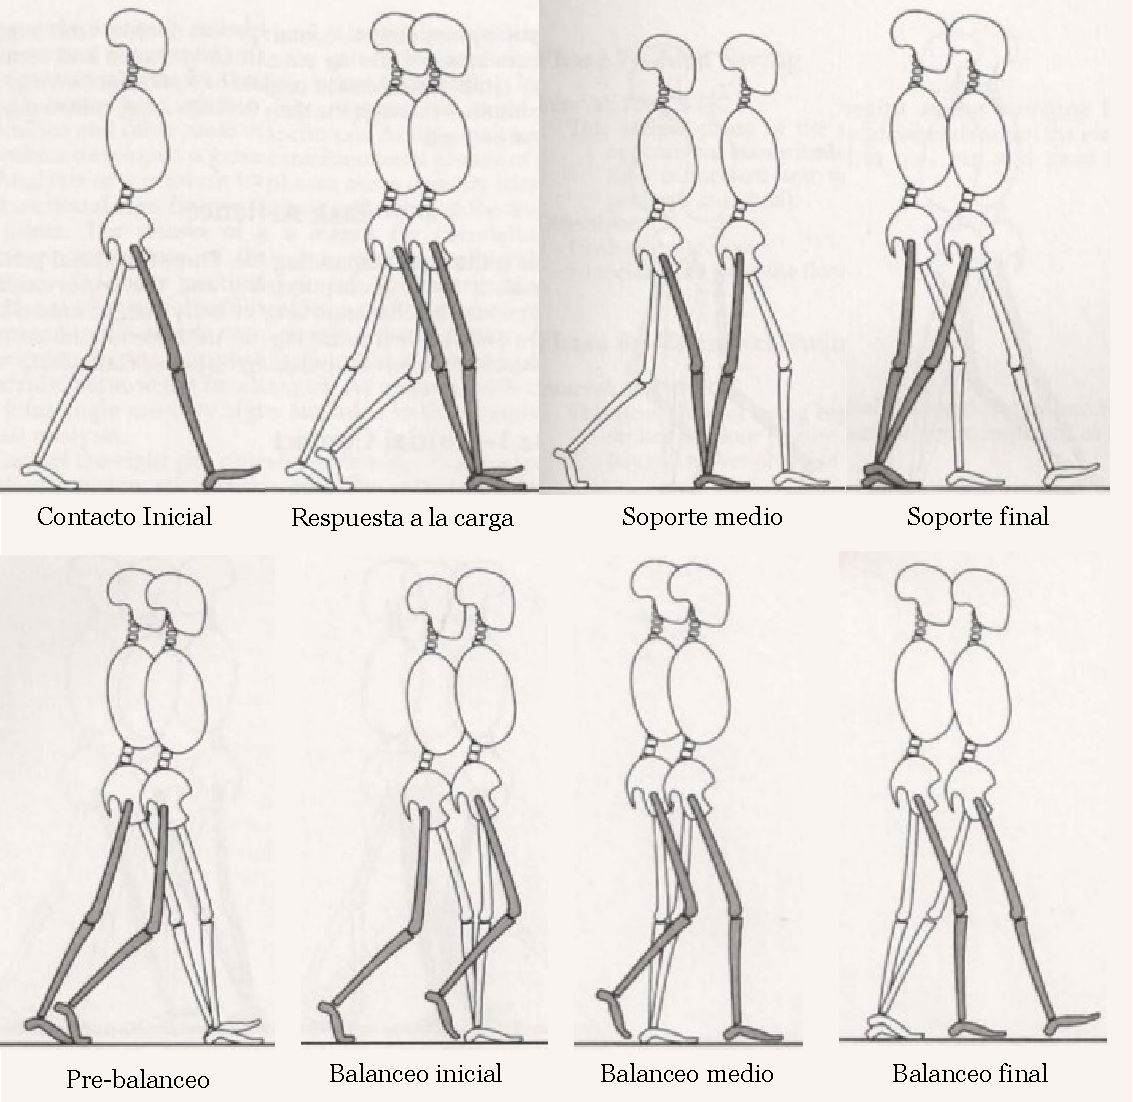
\includegraphics[width = \textwidth]{imagenes/ciclo_marcha}
    \caption{Ilustración del ciclo de la marcha, tomado de \citep{perry}}
    \label{fig:ciclo_marcha}
\end{figure}


A pesar del posible significado \emph{psicológico} de las fases detalladas en la tabla \ref{tab:ciclo_marcha} y la figura \ref{fig:ciclo_marcha}, si es posible encontrar un significado físico en el ciclo de la marcha. Considere la figura \ref{fig:menz_acc_ver}, tomada de \citep{menz}.

\begin{figure}
    \centering
    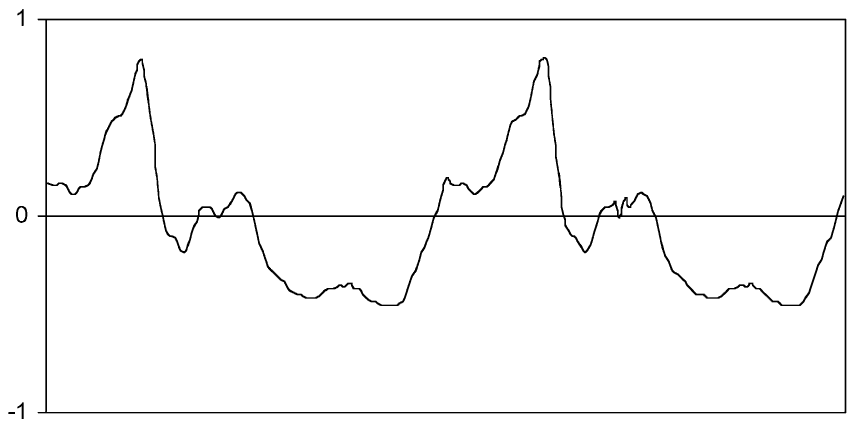
\includegraphics[width = 0.75\textwidth]{imagenes/menz_acceleration}
    \caption{Aceleración vertical de la cadera, tomado de \citep{menz}}
    \label{fig:menz_acc_ver}
\end{figure}

A grandes rasgos, el pico de mayor tamaño representan el momento donde se transfiere el peso de una pierna a la otra, existe en esa fase un tiempo muy corto donde el cuerpo está casi en caída libre (la gravedad es la principal fuerza de locomoción). Esto es seguido del contacto inicial y la aceptación de la carga. La valle largo y llano corresponde al fase de balanceo, donde una pierna se adelanta hacia la posición de contacto inicial.

Al utilizar sensores para recolectar datos de la marcha, se puede aplicar gran cantidad de herramientas matemáticas para caracterizar el movimiento e intentar encontrar \emph{patrones} útiles al diagnosticar condiciones clínicas. 





\section[Herramienta de diagnóstico]{Análisis de la marcha como herramienta de diagnóstico}

Tal como se menciona en la sección anterior, la marcha produce una serie de patrones, tanto en las variables cinemáticas como dinámicas. El análisis de dichos patrones puede utilizarse como herramienta de diagnostico. Tome por ejemplo un daño en los músculos pretibiales, principales encargados de elevar el piel al final de la fase de balanceo (figura \ref{fig:heel_rocker}). Sin la acción de este músculo la punta del pie, y no el talón, es el primero en hacer contacto con el piso, esto impide una transferencia de carga efectiva y aumenta el esfuerzo de la marcha.

Para compensar la función de los músculos pretibiales, el patrón de la marcha se ve modificado, un ejemplo es la marcha del personaje \emph{el vagabundo} de Charles Chaplin \footnote{En \url{https://www.youtube.com/watch?v=L277pNm3Y4w} se puede encontrar un extracto de Charles Chaplin interpretando al \emph{vagabundo}}. En este caso los cuadriceps hacen un esfuerzo extra para aumentar el ángulo de la rodilla, generando un pequeño latigazo, que permite un contacto inicial con la planta del pie (horizontal).

El patrón de la marcha de el personaje \emph{el vagabundo} parece ser una combinación de varias afectaciones, sin embargo su análisis permitiría encontrarlas y aplicar tratamientos correctivos: ejercicios, calzado ortopédico, operaciones. 

\begin{figure}
    \centering
    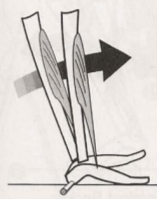
\includegraphics[width=0.2\textheight]{imagenes/heel_rocker}
    \caption{Función de los músculos pretibiales. Tomado de \citep{perry}}
    \label{fig:heel_rocker}
\end{figure}

Como estudio de caso, \cite{arif} plantea la hipótesis de que la edad afecta la estabilidad de marcha y propone analizar la entropía de la señal de aceleración, generada por un sensor colocado en la zona lumbar, para cuantificar la estabilidad de la marcha. Los resultados siguieren que la entropía de la marcha aumenta según la edad. Pero en general la entropía aumenta según la velocidad de la marcha, para compensar este hecho, las personas intentan optimizar la estabilidad al disminuir velocidad de la marcha. En general las personas mayores desarrollan una cadencia\footnote{Cadencia: cantidad de pasos por unidad de tiempo} menor que las personas jóvenes. 

Ahora bien, la edad no es el único factor que podría afectar la estabilidad de la marcha y su cadencia. Personas que sufren de enfermedades degenerativas, como esclerosis, Alzheimer, traumatismos cerebrales, entre otros, sufren de marcha inestable. Un estudio integral de la marcha, considerando otras variables, podría ayudar en el diagnóstico de enfermedades, cuantificar su afectación y proponer medidas para mejorar la calidad de vida del paciente. 

El análisis de marcha también puede ayudar a mejorar el rendimiento deportivo. Tal como señala \cite{perry}, los atletas empujar el funcionamiento normal del cuerpo hasta sus límites, esto se evidencia en el patrón de la marcha, generando mayores fuerzas en las articulaciones y arcos de movimiento más amplios. Entender cómo la práctica deportiva afecta los patrones de movimiento podría ayudar a disminuir el riesgo de lesiones y mejorar el desempeño.  






\section[Métodos de recolección]{Métodos de recolección de datos}

En el estado del arte, se pueden identificar los siguientes grupos de métodos para la recolección de datos: dispositivos \emph{wearables}, dispositivos ópticos de cámaras, marcadores activos y marcadores pasivos. El primer grupo tiene como ventaja ser dispositivos baratos y pequeños, el paciente bajo estudio puede llevarlos sobre sí y continuar con sus actividades diarias, como desventaja se pierde toda información sobre la localización del paciente. El segundo grupo tiene como desventaja necesitar un espacio físico muy limitado para realizar la prueba, el equipo es caro, pero suele ser muy preciso y su principal ventaja: permite conocer la posición, velocidad y aceleración de cada segmento del cuerpo. 

\subsection{Dispositivos \emph{wearables}}

Tradicionalmente, consisten de acelerómetros y (opcional) giroscopios, los cuales son manejados por un micro-controlador, los datos se almacenan internamente o son transmitidos a un computador por algún medio.

\cite{krigslund} desarrolló un método para conocer la orientación de segmentos rígidos utilizado un dispositivo RFID con antenas bipolares, al ser pasivos, estos dispositivos podrían utilizarse por largo tiempo, sin embargo se necesita equipo alrededor para recolectar los datos. 

\cite{yuan} presenta un método con el cual se puede conocer la posición del usuario, utilizando un arreglo de 8 IMUs (acelerometro+giroscopio) colocados sobre el cuerpo, esto amplía significativamente la utilidad de estos métodos de recolección de datos. 

A pesar de estos avances, en el estado actual, los sistemas de captura de movimiento con dispositivos \emph{wearable} pierden mucha información importante sobre el ciclo de la marcha, esto podría cambiar con el desarrollo de dispositivos integrados en la ropa del paciente, tal como propone \cite{menguc}.

\subsection{Cámaras digitales} 

Al ser dispositivos muy baratos y de procesamiento accesible, son muy utilizadas. Se suelen colocar varias cámaras en diversas configuraciones, por ejemplo \cite{hoang} las coloca viendo el mismo objeto una al lado izquierdo y otra al derecho, mientras tanto \cite{li} las coloca ortogonalmente. 

A pesar de su bajo costo y sencillez, estos dispositivos tiene menor precisión que los basados en marcadores.

\subsection{Sistemas ópticos}

Este método es muy utilizado en animación digital. Dispositivos ópticos (Algún tipo de cámara) se colocan cubriendo todo un espacio, al paciente se le colocan sobre el cuerpo un conjunto de \emph{marcadores}, pueden ser activos o pasivos. Las dispositivos debe colocarse de manera que ningún marcados quede oculto, sin importar la pose del paciente. La figura \ref{fig:pris_mocap} muestra el sistema de captura óptica del movimiento (MoCap) del Pris-Lab, Escuela de Ingeniería Eléctrica, Universidad de Costa Rica. 

Comúnmente, estos métodos son muy costosos y necesitan de software privativo especializado para renderizar un esqueleto a partir de los marcadores, sin embargo tienen la ventaja de ser muy precisos. 
%\begin{figure}
%    \centering
%    \includegraphics[width = 0.6\textwidth]{images/pris_mocap}
%    \caption{Sistema MoCap del Pris-Lab, UCR}
%    \label{fig:pris_mocap}
%\end{figure}

\section[Software disponible]{Software disponible para estudios sobre la marcha}

En muchos casos, los estudios sobre la marcha se realizan con software específico para el experimento, desarrollado en alguna plataforma como Matlab (este es el caso de la mayoría de trabajos analisados). Por ejemplo \cite{menz} utiliza SPSS, un software de análisis estadístico predictivo. \cite{takahiro}, por ejemplo, utiliza nMotion Musculous de NAC Image Technology, con lo cual calcula la fuerza de activación de cada músculo y después hace un análisis estadístico, no especifica en cual plataforma, pero podría ser incluso en una hoja de cálculo. 

En un ambiente clínico, existen programas especializados en ayudar al practicante en el diagnóstico y seguimiento de las dificultades motoras. Por ejemplo se tiene 3D Gait, TEMPLO Contemplas, Medical Motion Pro-Trainer Motion analysis, Motion Monitor Gait Analysis, entre otros.  

Hasta el momento, no se ha encontrado un software libre que permita realizar estudios de la marcha. 


